\section{Use Cases and HCI Scenarios}
\label{sect:use_cases_and_hci_scenarios}
% Persona 1
\subsection{HCI Persona 1}
\label{sect:hci_persona_1}

\begin{Parallel}[v]{0.48\textwidth}{0.48\textwidth}
\ParallelLText{
\begin{minipage}{0.40\textwidth}
    \begin{figure}[H]
        \begin{centering}
        	\colorbox{lightgray}{{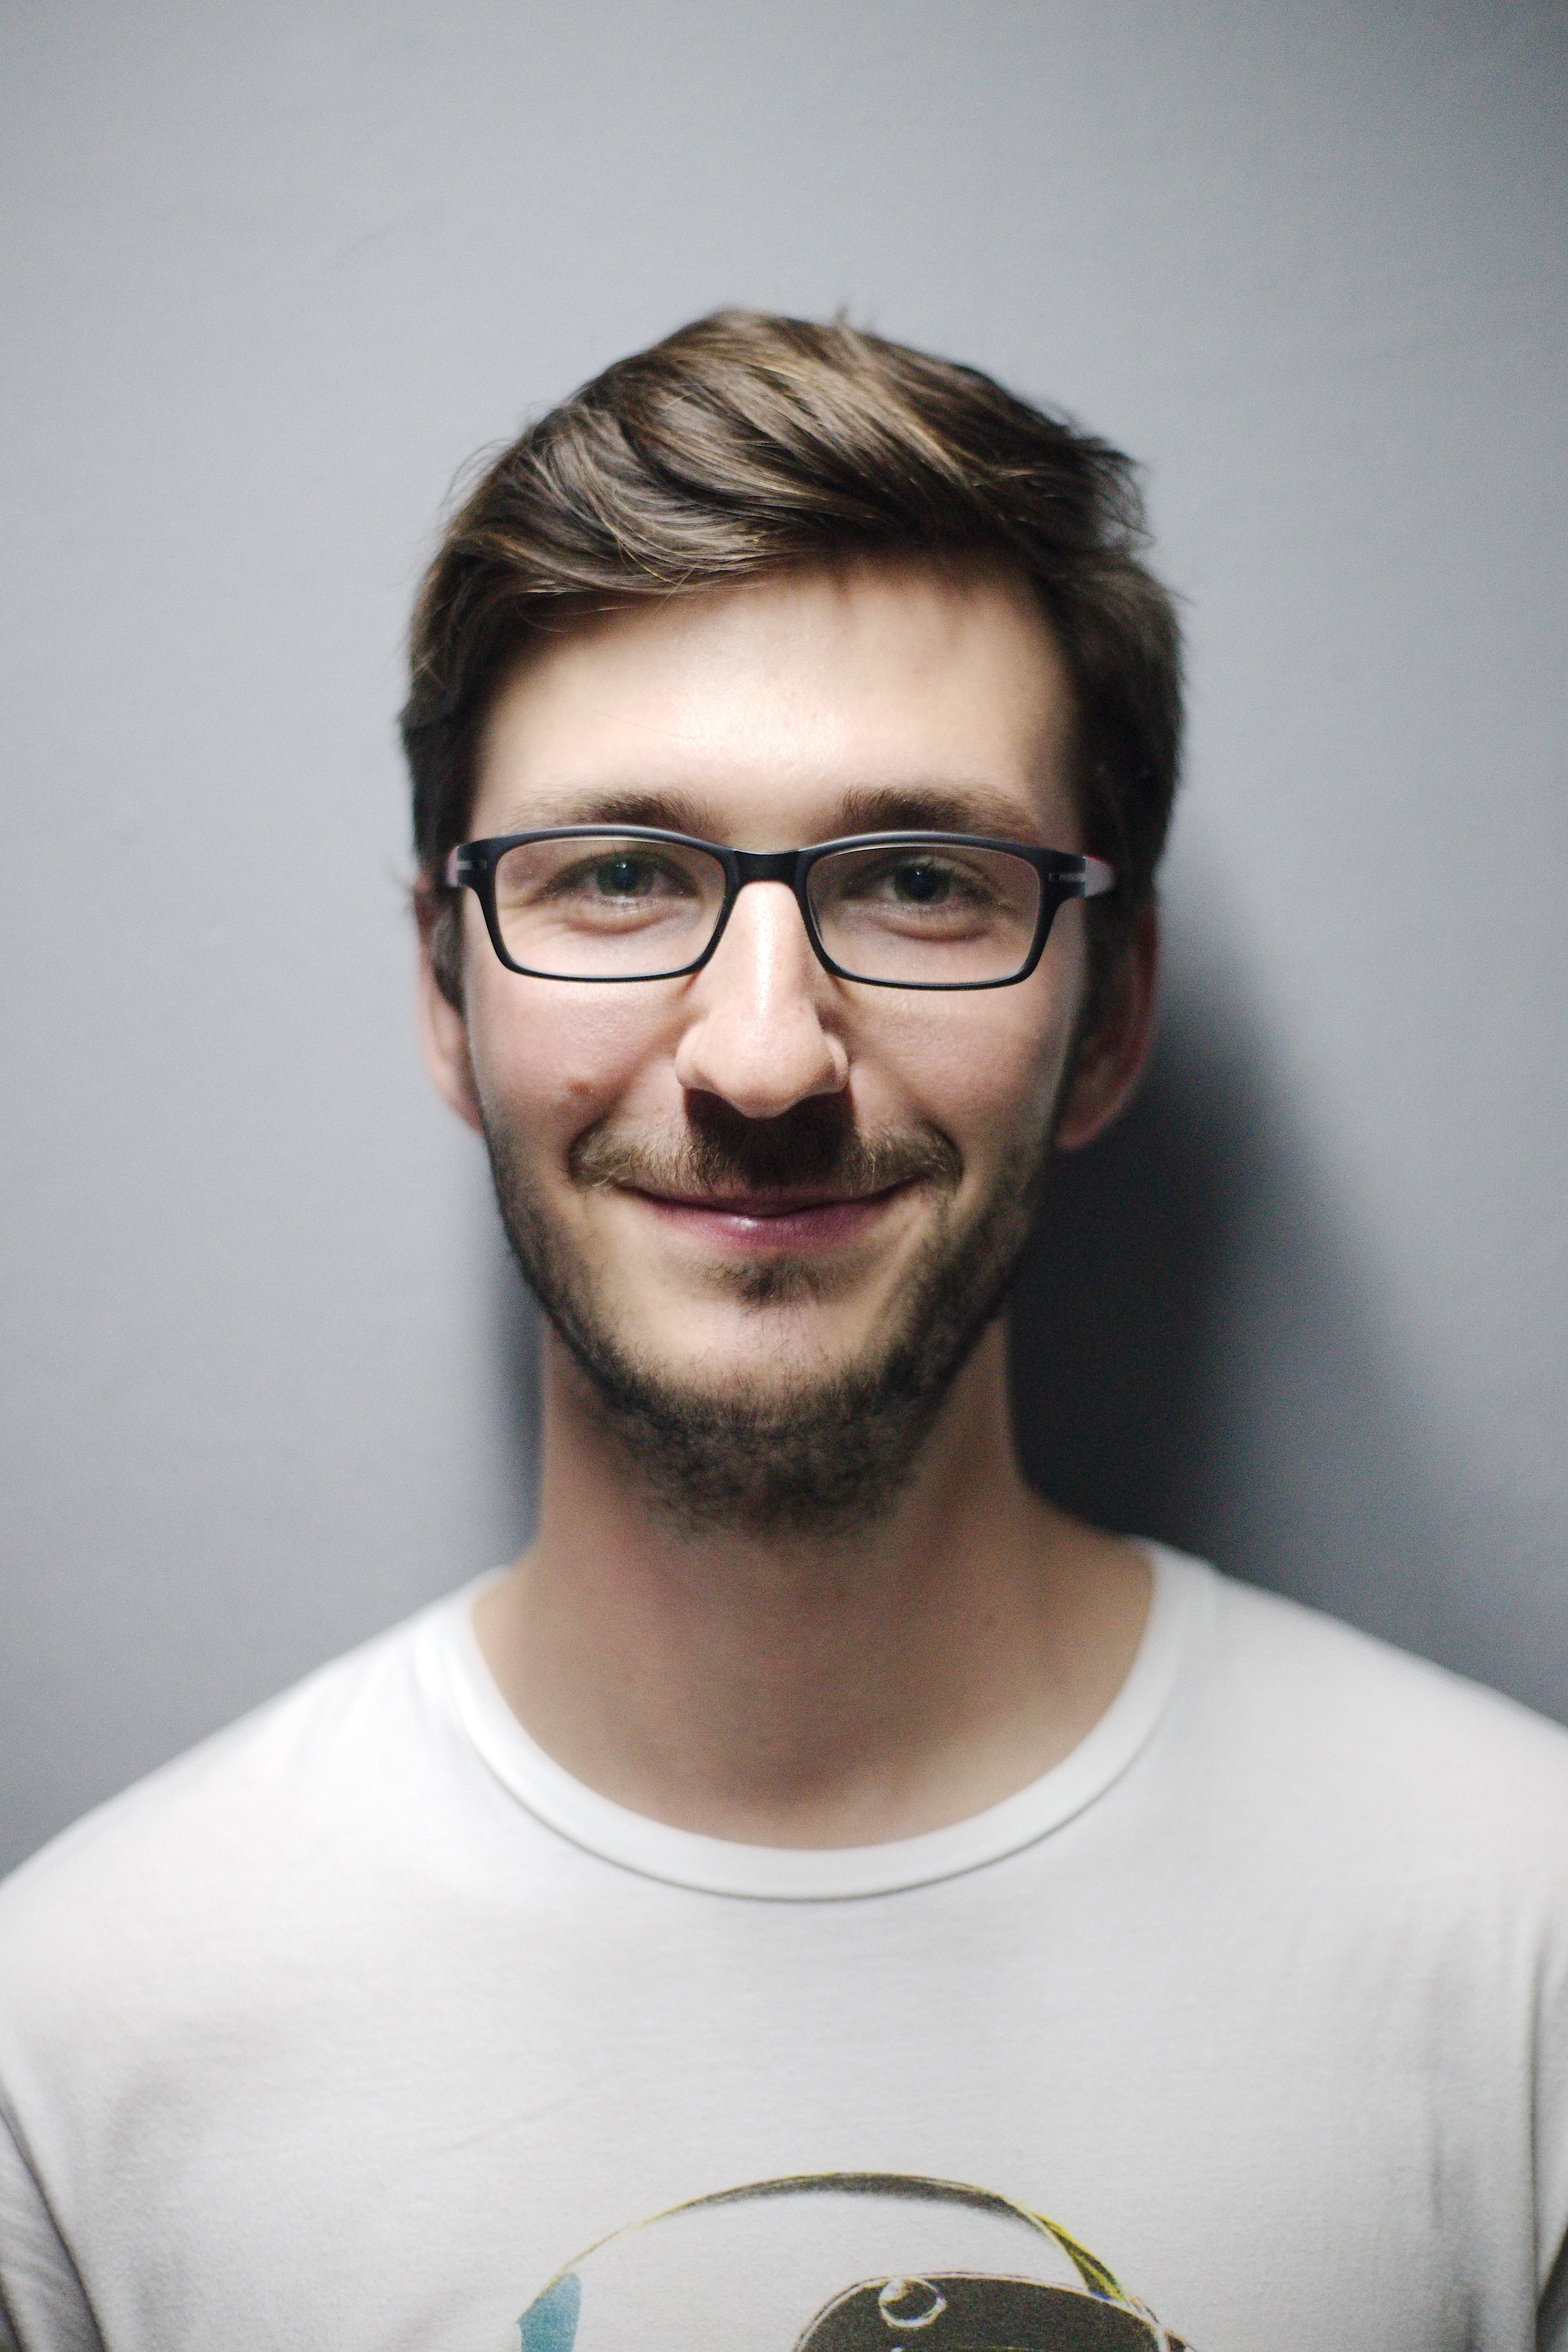
\includegraphics[width=0.80\linewidth, height=1.00\linewidth]{personas/persona_1.jpg}}}
        	\caption{A photo of a fictional male persona for the PyBank application~\cite{PEXELS_MALE_PERSONA:4}.}
        	\label{fig:persona_1}
        \end{centering}
    \end{figure}
    \begin{centering}
        \begin{itemize}[leftmargin=*]
            \item {\textbf{Fictional Name:}~John Doe}
            \item {\textbf{Job Title:}~Accountant}
            \item {\textbf{Demographics:}
                \begin{itemize}[leftmargin=*]
                    \item {\textbf{Age:}~26}
                    \item {\textbf{Marital Status:}~Single}
                    \item {\textbf{Degree:}~B.A. Accounting}
                \end{itemize}
            \item {\textbf{Goals and Tasks:}
                \begin{itemize}[leftmargin=*]
                    \item {Perform accounting services for local companies using PyBank's desktop client.}
                    \item {Learn PyBank's interface in-depth to become a power user.}
                \end{itemize}}}
        \end{itemize}
    \end{centering}
\end{minipage}}
\ParallelRText{\begin{minipage}{0.40\textwidth}
    \subsubsection*{Environment}
    \begin{centering}
        John, an accountant for a local firm, typically performs work on a desktop computer system. He's a busy individual, handling the accounts of both local and widespread businesses. John's spends the majority of his time performing financial computations, answering phones, and writing complex reports with visualizations. Sometimes, when John has to travel, he performs work-related tasks on a laptop computer system instead of other mobile alternatives because he always wants to have the highest performance while working for his clients.
    \end{centering}
    \subsubsection*{Scenario}
    \begin{centering}
        John recently began merging all of his clients accounts into to the PyBank desktop application. During a recent trip, where internet activity was scarce, John was prepared. Thanks to Pybank, John was still able to perform accounting tasks for his clients that were processed, recorded, and once he regained internet access, updated in the cloud. PyBank's flexibility and accessibility allowed John to perform work that other individuals were restricted from performing with traditional banking systems.
        \vspace{10mm}
    \end{centering}
\end{minipage}}
\ParallelPar
\end{Parallel}

\newpage

% Persona 2
\subsection{HCI Persona 2}
\label{sect:hci_persona_2}

\begin{Parallel}[v]{0.48\textwidth}{0.48\textwidth}
\ParallelLText{
\begin{minipage}{0.40\textwidth}
    \begin{figure}[H]
        \begin{centering}
        	\colorbox{lightgray}{{
\includegraphics[width=0.80\linewidth, height=1.00\linewidth]{personas/persona_2.jpg}}}
        	\caption{A photo of a fictional female persona for the PyBank application~\cite{PEXELS_FEMALE_PERSONA:4}.}
        	\label{fig:persona_2}
        \end{centering}
    \end{figure}
    \begin{centering}
        \begin{itemize}[leftmargin=*]
            \item {\textbf{Fictional Name:}~Jane Doe}
            \item {\textbf{Job Title:}~Financial Analyst}
            \item {\textbf{Demographics:}
                \begin{itemize}[leftmargin=*]
                    \item {\textbf{Age:}~28}
                    \item {\textbf{Marital Status:}~Married}
                    \item {\textbf{Degree:}~B.A. Finance}
                \end{itemize}
            \item {\textbf{Goals and Tasks:}
                \begin{itemize}[leftmargin=*]
                    \item {Manage personal finances using PyBank's desktop client from the comfort of home.}
                    \item {Utilize PyBank's financial visualizations for insights and reports.}
                \end{itemize}}}
        \end{itemize}
    \end{centering}
\end{minipage}}
\ParallelRText{\begin{minipage}{0.40\textwidth}
    \subsubsection*{Environment}
    \begin{centering}
        Jane is a freelance financial analyst who prefers to work remotely. Her work is generally done on a laptop since she often enjoys working at the coffee shop or other social venues. Jane prefers summarized data visualizations that help her make quick analytical interpretations.
    \end{centering}
    \subsubsection*{Scenario}
    \begin{centering}
        Recently, at Jane's favorite local coffee shop, Jane decided that she wanted to analyzer her families' personal finances and present the results to her husband in an easy to understand manner. With this goal in mind she focused on creating histograms and pie charts for categorical data and a line graph for plotting her families spending over time. With the help of PyBank, she was able to generate these visualizations and produce a summary of her families spending in no time, all while consuming her favorite coffee drink!
        \vspace{43.5mm}
    \end{centering}
\end{minipage}}
\ParallelPar
\end{Parallel}

\newpage

\subsection{Use Case Diagram}
\label{sect:use_case_diagram}

Listed below are brief descriptions of eleven use cases that describe a sequence of a sequence of actions that can be performed by a PyBank customer (the end-user) interacting with PyBank, an interactive desktop client banking application. These use cases are further depicted in Figure~\ref{fig:use_case} shown below after the use case descriptions.

\begin{enumerate}[itemsep=1mm, parsep=0pt]
    % UC_01
    \item {\textbf{CreatePyBankAccount~(UC\_01):}~A PyBank customer can create an account from PyBank's main application window by selecting the~\texttt{\textcolor{red}{Create An Account}}~button.}
    % UC_02
    \item {\textbf{DepositSavingsAccount~(UC\_02):}~A PyBank customer can deposit money into an existing savings account by selecting the~\texttt{\textcolor{red}{Make A Deposit}}~button from the Savings Account application window.}
    % UC_03
    \item {\textbf{DepositCheckingAccount~(UC\_03):}~A PyBank customer can deposit money into an existing checking account by selecting the~\texttt{\textcolor{red}{Make A Deposit}}~button from the Checking Account application window.}
    % UC_04
    \item {\textbf{SignIntoPyBankAccount~(UC\_04):}~A PyBank customer can sign in to an existing account from PyBank's main application window by selecting the~\texttt{\textcolor{red}{Sign In}}~button.}
    % UC_05
    \item {\textbf{WithdrawSavingsAccount~(UC\_05):}~A PyBank customer can withdraw money from an existing savings account by selecting the~\texttt{\textcolor{red}{Make A Withdrawal}}~button from the Savings Account application window.}
    % UC_06
    \item {\textbf{AddCheckingAccount~(UC\_06):}~A PyBank customer can request a checking account from PyBank by selecting the~\texttt{\textcolor{red}{Add A Checking Account}}~button from the main application window. A PyBank customer may have~\textbf{\underline{one}}~checking account per PyBank account.}
    % UC_07
    \item {\textbf{WithdrawCheckingAccount~(UC\_07):}~A PyBank customer can withdraw money from an existing checking account by selecting the~\texttt{\textcolor{red}{Make A Withdrawal}}~button from the Checking Account application window.}
    % UC_08
    \item {\textbf{ViewSavingsAccountGraphs~(UC\_08):}~A PyBank customer can view graphical charts related to their savings account by selecting the~\texttt{\textcolor{red}{View Graphs}}~button from the Savings Account application window.}
    % UC_09
    \item {\textbf{ViewCheckingAccountGraphs~(UC\_09):}~A PyBank customer can view graphical charts related to their checking account by selecting the~\texttt{\textcolor{red}{View Graphs}}~button from the Checking Account application window.}
    % UC_10
    \item {\textbf{AddSavingsAccount~(UC\_10):}~A PyBank customer can request a savings account from PyBank by selecting the~\texttt{\textcolor{red}{Add A Savings Account}}~button from the main application window. A PyBank customer may have~\textbf{\underline{one}}~savings account per PyBank account.}
    % UC_11
    \item {\textbf{SignOutOfPyBankAccount~(UC\_11):}~A PyBank customer can sign out of an existing account from PyBank's main application window by selecting the~\texttt{\textcolor{red}{Sign Out}}~button from the navigation menu.}
\end{enumerate}

\newpage

\begin{figure}[H]
	\begin{centering}
	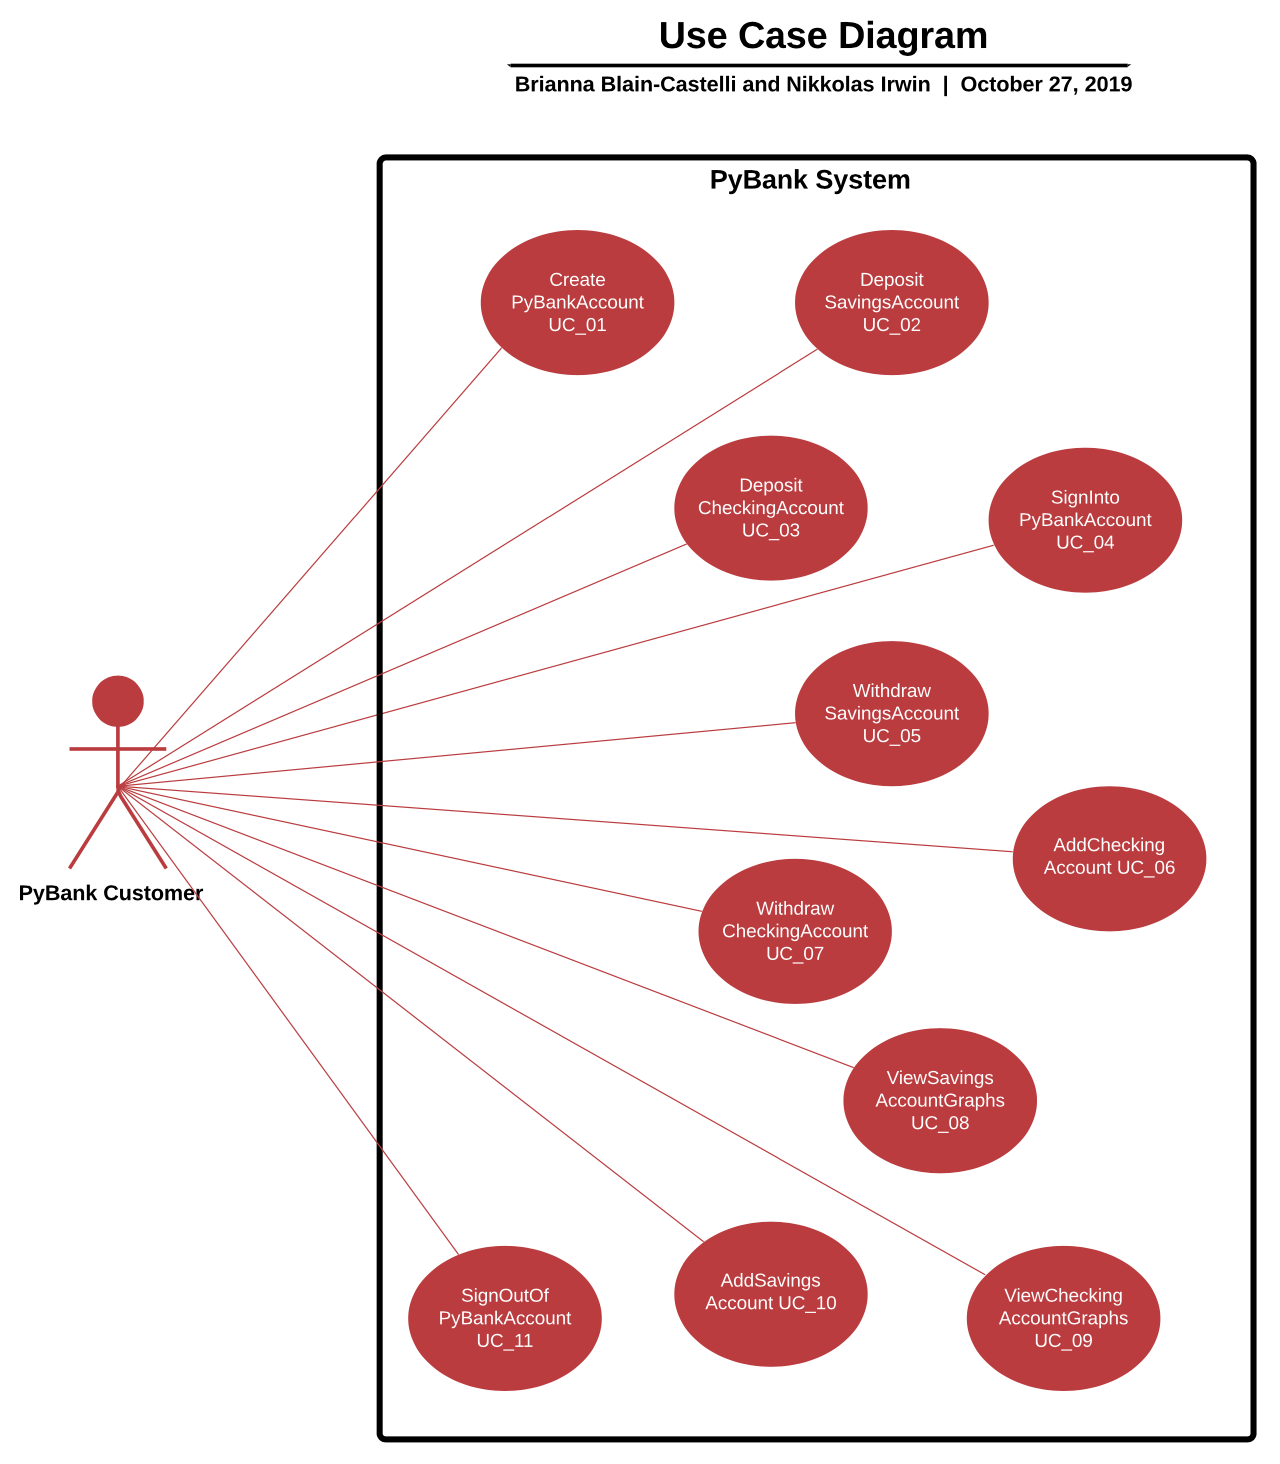
\includegraphics[width=1.00\linewidth, height=1.10\linewidth]{diagrams/use_case_diagram.png}
	\caption{A use case diagram, created using Lucidchart~\cite{LUCID_CHART:5},~for PyBank, an interactive desktop client banking application.}
	\label{fig:use_case}
	\end{centering}
\end{figure}


% EOF